\documentclass{article}

\usepackage{neurips_2019_author_response}

\usepackage[utf8]{inputenc} % allow utf-8 input
\usepackage[T1]{fontenc}    % use 8-bit T1 fonts
\usepackage{hyperref}       % hyperlinks
\usepackage{url}            % simple URL typesetting
\usepackage{booktabs}       % professional-quality tables
\usepackage{amsfonts}       % blackboard math symbols
\usepackage{nicefrac}       % compact symbols for 1/2, etc.
\usepackage{microtype}      % microtypography
\usepackage{todonotes}
\usepackage{caption}
\usepackage{bm}

\begin{document}

%#3comparison of performance with the original models on a set of arithmetic tasks (significance: medium to low)

\paragraph{Why does the NALU perform great in the original paper?} %#3why does the multiplication perform satisfactory in the original paper, but fails in this paper. %#3 the paper does a superb analysis of the issues, but it is unclear whether these issues make the original model unusable (from the original paper it seems that is not the case) and how difficult do they make it train (what is the standard number of iterations NALU is trained for)?
We have contacted the authors of the NALU paper, unfortunately they have been unable to provide any specific details about the models or experiments.
As such, we firmly believe our implementation and experiments are identical to theirs.
Our experience with NALU is that convergence only happens for a lucky initialization.
In the NALU paper no analysis of ``success rate'' was done and we believe their results are heavily cherry-picked.
However, as we do not think speculation of scientific integrity is appropriate in a paper we have omitted such comments. %#3how come NALU performs great in the original paper, but is often worse than the linear model in this paper? The difference wrt the results in the original paper needs to be properly explained in the paper.
\textit{Why is the NALU worse than the linear model?} The NALU shares weights between the $\mathrm{NAC}_{+}$ and $\mathrm{NAC}_{\bullet}$ layers.
By comparing it to a NALU without weight sharing we find that weight sharing makes addition harder (4\% success rate), but multiplication feasible. %#3the resulting experiments are specific to pick out the disadvantages of the original model 
\textit{Are the experiments designed to show a disadvantage with NALU?} Our experiments are identical to the ``simple function task'' in the NALU paper.
Only \texttt{input\_size} is defined in the original paper so we choose to vary all parameters of the task in order to test consistency of learning.

\vspace{-0.3cm} \paragraph{Is the comparison between NMU and $\mathrm{NAC}_{\bullet}$ unfair?} %#1It's not surprising to me that the proposed multiplication unit NMU outperforms $NAC_\cdot$, since $NAC_\cdot$ is targeting a more ambitious division operation as well, so the comparison is unfair. %#3Comparisons to the original model under the set of conditions of the original paper, and slowly showing/developing the issues of that model, i.e. starting with a fair comparison and then showing where the original model fails.\\
Maybe, it is true that the NMU model, unlike $\mathrm{NAC}_{\bullet}$, does not support division.
On the other hand the NMU can model inputs in the negative range.
To make a more fair comparison we have added two additional units; $\mathrm{NAC}_{\bullet, \sigma}$ that only supports multiplication by using $W = \sigma(\hat{W})$ in the $\mathrm{NAC}_{\bullet}$, and $\mathrm{NAC}_{\bullet, \mathrm{NMU}}$ which is a variant of $\mathrm{NAC}_{\bullet}$ using linear weights \& bias regularization identically to the NMU model.
%Figure \ref{fig:sft-hidden-size} illustrates that both variations improve upon $\mathrm{NAC}_{\bullet}$, but not enough to be better than NMU. %#3Balance the conclusion, as it currently states the advantaged of NAU and NMU without mentioning their drawbacks, which seem significant wrt NALU.\\
\textit{The conclusion currently states the advantaged of NAU and NMU without mentioning their drawbacks.} Good point, we have fixed that. Although, please note that the original paper does not solve division and that neither the $\mathrm{NAC}_{\bullet, \sigma}$ or $\mathrm{NAC}_{\bullet, \mathrm{NMU}}$ supports division or inputs in the negative range. %#3Also, the presented models specialize for three arithmetic operations where the original model was tested on three more operations. #3Are these models applicable to those operations too?
\textit{$\mathrm{NAC}_{\bullet}$ supports $\sqrt{x}$ and $x^2$, does NMU support those?} NMU supports $x^2$, in the same way as $\mathrm{NAC}_{\bullet}$ does, by using $x^2 = x \cdot y$,  where $y = x$.
NMU and $\mathrm{NAC}_{\bullet, \mathrm{NMU}}$ does not support roots such as $\sqrt{x}$, we will mention this in the revision.

\vspace{-0.3cm}\begin{figure}[h]
\centering
\begin{minipage}{.48\textwidth}
  \centering
  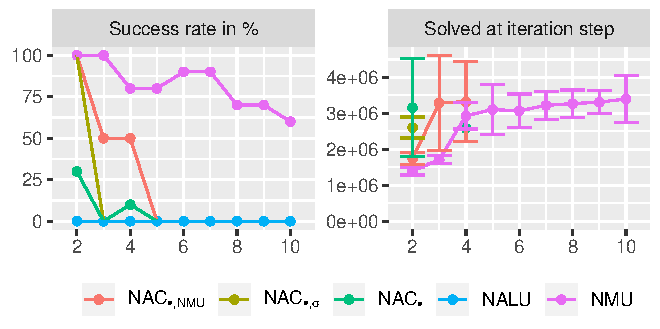
\includegraphics[width=\linewidth,trim={0 0 0 0},clip]{results-author-response/simple_function_static_mul_hidden_size.pdf}
  \vspace{-0.65cm}
  \captionof{figure}{Shows effect of increasing hidden size by adding redundant hidden units in the arithmetic task. Sparsity error is excluded due to space constraints.}
  \label{fig:sft-hidden-size}
\end{minipage} \hspace{0.4cm}
\begin{minipage}{.48\textwidth}
  \centering
  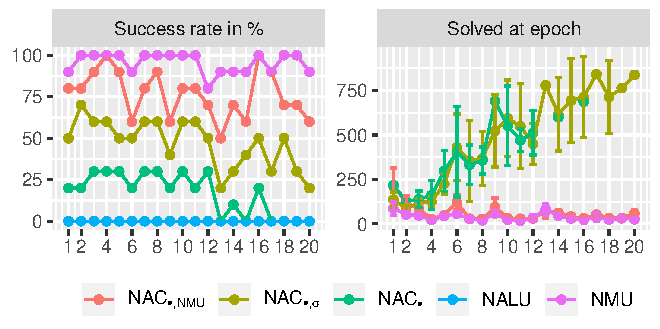
\includegraphics[width=\linewidth,trim={0 0 0 0},clip]{results-author-response/sequential_mnist_prod_long.pdf}
  \vspace{-0.65cm}
  \captionof{figure}{Multiplication of MNIST images. X axis is extrapolation to a given sequence length images, trained on sequence length 2. Sparsity error excluded for space.}
  \label{fig:mnist}
\end{minipage}
\end{figure}

\vspace{-0.5cm} \paragraph{More experiments} In figure \ref{fig:sft-hidden-size} we test our theoretical finding that $\mathrm{NAC}_{\bullet}$ is unstable for a large hidden size (equation 11).
Additionally, we have added the MNIST experiment from the original paper where we test on multiplication instead of addition.
The MNIST experiment evaluates how well a deep neural network can backpropagate through the $\mathrm{NAC}_{\bullet}$ or the NMU layer.
The results in figure \ref{fig:mnist} show that the NMU converges more consistently and faster, which might indicate that the partial linearity in NMU makes for easier backpropergation. \textit{The novelty is only limited to the theoretical analyses of NALU and a new parameterization.} As we found that the NALU rarely converges on their own tasks we choose to focus our efforts to understanding why it does not work and invent a new neural units based on those theoretical findings rather than creating new experimental settings.
%We hope that these additional experiments will convince you that our contributions are worth of publication.

\vspace{-0.3cm} \paragraph{Is $\bm{\mathbb{E}[z_{h_l}] = 0}$ necessary for optimization?} $E[z_{h_l}] = 0$ is a desirable property and not a theoretical necessity.
We used this desirable property as an inspiration when designing the NMU, which we find converges more often and optimizes faster in our experiments.
Our new comparison with $\mathrm{NAC}_{\bullet, \mathrm{NMU}}$ directly test the effect of this property by increasing \texttt{hidden\_size}.
We will emphasize that $E[z_{h_l}] = 0$ is only a desirable property in our revision.

\vspace{-0.3cm} \paragraph{Other questions.} \textit{Would weight clipping have saturation issues?} No, the $\mathcal{R}_{oob}$ regularizer provides gradient outside $[0,1]$. Also, for simplicity our latest revision replaces $\mathcal{R}_{oob}$ with a truncation in each iteration.
\textit{Does regularization in the NALU help?}
We did a lot of initial experiments trying to fix the NALU including adding regularization. Our conclusion was that the gating mechanism is a critical issue superseding all other concerns (see L77-81).
\textit{Are the assumptions of splitting the NALU worth the effort?} NALU has its own issues, regarding the gating mechanism. However, we believe that before the gating issue can be solved, the subunits needs to converge consistently.
We leave the gating mechanism issues of the NALU for future research.
\textit{Why did you chose $\lambda_{bias}$ in this way?} Post submission, we found that learning interpolation and then sparsifying to learn extrapolation are two different optimization problems. Only the latter requires regularization. In our revision the bias regularizer is now scaled with a spline function (shape similar to ReLU6).
\textit{Is the parameter sparsity a necessity?} For multiplication it is a requirement. For addition and subtraction it helps with interpretability. 
\textit{Does the $\mathrm{NAC}_{+}$ need fixing?} The NAU converges faster, uses half the parameters, and bias towards discrete weights. We believe these contributions are noteworthy, but agree that they are minor.

\vspace{-0.3cm} \paragraph{Minor comments and typos.} Thanks for noticing, these issues have been fixed in our revision.

% \paragraph{Final words.} We think the NALU have strong signs of scientific misconduct. We find that very disapointing. Our primary goal have been to fix the issues and have a strong scientific integrity.

\end{document}